\chapter{Benchmarks en Experimenten}
% \chaptermark{Een kortere titel voor de paginahoofding (verschillend van titel in TOC)}

\todo[inline,caption={}]{Terminologie?

\begin{itemize}
	\item Object (geretourneerde gegevens.) <-> OID's (kunnen subtakken zijn van meerdere OID's)
	\item SNMP Data Retriever
	\item Relevante OID's/objecten/gegevens
\end{itemize}

}

\section{Kleinschalige benchmarks en experimenten}

\todo[inline]{Schrijf een inleiding. \\
Enerzijds de Virtual Box opstelling. Anderzijds heb je ook de iMinds switchen. Ten slotte de profiler.}

\todo[inline]{Eigenlijk maakt het weinig uit om wat voor soort toestellen het gaat:
alhoewel de applicatie voornamelijk bedoeld is voor netwerkapparatuur, voor onze testen hebben we enkel een noodzaak aan voldoende gegevens die via SNMP kunnen opgevraagd worden.}

\subsection{VirtualBox}

\todo[inline]{Betere titel! Virtuele testopstelling van een handvol switches.}

\todo[inline, caption={}]{
Bespreking originele testopstelling van Wouter Tavernier? \\
Specs \\
Software(config)

\begin{itemize}
	\item screen (niet geinstalleerd)
	\item sudo
	\item snmpd
	\item snmp
	\item snmp-mibs-downloader
	\item bridge, lldp...
\end{itemize}


}

De eerste testopstelling bestaat uit vier virtuele machines die switches in een netwerk nabootsen.
Als virtualisatieplatform wordt er gebruik gemaakt van \textit{Oracle VM VirtualBox} (verder gewoon VirtualBox genoemd).
VirtualBox is vrij te verkrijgen voor alle gangbare besturingssystemen en is bovendien open-source.

\subsubsection{Hardwareconfiguratie}

Het gastheerbesturingssysteem is een 64-bit versie van Windows 7.
Windows en VirtualBox zijn geïnstalleerd op een SSD, maar de virtuele machines zelf staan op een magnetische harde schijf.

Aan elke node wordt 256 MB geheugen en een CPU kern (van een Intel Core i7 3610QM processor) toegewezen.
Op de nodes wordt een minimale versie van Debian 7 geïnstalleerd, zonder grafische schil.
Hierdoor is zelfs 256 MB een ruime luxe voor de nodes: na het opstarten van een node wordt er amper 70MB geheugen gebruikt.

Alle toestellen zijn rechtstreeks met elkaar verbonden in een privénetwerk.
Via \gls{nat} kunnen ze via de gastheer toch nog het internet bereiken.
Dit werd bewerkstelligd met de \textit{NAT Network mode},
een nieuwe feature in VirtualBox die nog niet in de documentatie staat maar wel kort beschreven wordt in een nieuwspost (zie\cite{vbox-nat-network-mode}).
Ter vergelijking:
\textit{NAT mode} laat gastsystemen toe om met het internet te communiceren via \gls{nat} maar zitten elk in een apart privénetwerk en kunnen dus niet met elkaar praten.
\textit{Host-only mode} laat gastsystemen met elkaar (en het gastheersysteem) communiceren door ze in een gezamelijk privénetwerk te plaatsen, 
maar communicatie met het internet is niet mogelijk.

\subsubsection{Softwareconfiguratie}

Hieronder leggen we kort stap voor stap uit hoe je op een Debianinstallatie de nodige SNMP software kunt installeren en configureren.
De uitleg is zeer is zeer beknopt gehouden en dient enkel om je op weg te helpen.
In de testopstelling werden de nodes ook nog geconfigureerd als switches die het \gls{stp} draaien alsook het \gls{lldp}.
Deze extra protocollen bieden informatie aan die via SNMP opgevraagd kan worden en zijn ook gegevens die in een realistische situatie opgevraagd kunnen worden.
De configuratie als switch en van LLDP wordt hier echter niet besproken. \todo{Dit kan eventueel als bijlage uitgelegd worden.}

Zoals gezegd worden alle nodes voorzien van een minimale Debian 7 installatie.
Dit wil zeggen dat er geen extra softwarepakketten worden geselecteerd bij installatie.

In de veronderstelling dat het internet werkt beginnen we na de installatie met het updaten van het systeem en het installeren van \textit{sudo}:

\begin{lstlisting}[language=bash]
# apt-get update
# apt-get upgrade
# apt-get install sudo
\end{lstlisting}

Maak een gebruiker aan en zorg ervoor dat je sudo rechten hebt met behulp van het \textit{visudo} commando of door je gebruiker toe te voegen aan de \textit{sudo} groep.

\begin{lstlisting}[language=bash]
# visudo
# usermod -a -G sudo <jouw gebruikersnaam>
\end{lstlisting}

Dan installeren we de snmp \textit{daemon} die zal antwoorden op SNMP requests.
Om te testen is het ook interessant om de client-side SNMP tools te installeren alsook een tool om de belangrijkste \glspl{mib} te downloaden.
Met die \glspl{mib} worden numerieke \glspl{oid} omgezet naar de leesbare tekstuele voorstelling.

Debian laat standaard niet toe dat niet-vrije (non-free) software\footnote{
	Dit is software die niet volledig vrij is maar op een of andere manier beperkt wordt door zijn licentie. De eisen die gesteld worden aan vrije software voor Debian zijn te vinden in de Debian Free Software Guidelines (DFSG)\cite{dfsg}\cite{dfsg-wiki}.}
geïnstalleerd wordt. De \textit{snmp-mibs-downloader} tool is daar een voorbeeld van.
Om dit toch toe te laten moet je voor elke lijn in /etc/apt/sources.list het non-free component achteraan toevoegen.
Dan krijg je zoiets:

\begin{lstlisting}[language=bash]
deb http://ftp.belnet.be/debian wheezy main non-free
deb-src http://ftp.belnet.be/debian wheezy main non-free
\end{lstlisting}

Nu kunnen we wel snmp-mibs-downloader en de andere tools installeren.

\begin{lstlisting}[language=bash]
$ sudo apt-get install snmpd snmp snmp-mibs-downloader
\end{lstlisting}

Het volgende commando zal de \glspl{mib} downloaden:

\begin{lstlisting}[language=bash]
$ sudo download-mibs
\end{lstlisting}

Het gebruik van de \glspl{mib} kun je aanzetten door de volgende regel in commentaar te zetten in het bestand /etc/snmp/snmp.conf:

\begin{lstlisting}[language=bash]
mibs :
\end{lstlisting}

Om \textit{snmpd} te configureren kun je gebruik maken van het \textit{snmpconf} commando die op interactieve wijze configuratiebestanden aanmaakt.
We moeten ook nog de locatie van de \gls{mib}-bestanden opgeven. Voeg daarom het volgende toe aan /etc/default/snmpd:

\begin{lstlisting}[language=bash]
export MIBS=/usr/share/mibs
\end{lstlisting}

Vervolgens herstarten we snmpd om de nieuwe configuratie in te laden.

\begin{lstlisting}[language=bash]
$ sudo /etc/init.d/snmpd restart
\end{lstlisting}

We kunnen testen of alles werkt met het volgende:

\begin{lstlisting}[language=bash]
$ snmpwalk -v1 -cpublic localhost mib-2
\end{lstlisting}

\todo[inline]{Verder eventueel: bridge configuratie, LLDP}

\todo[inline]{SNMP Data Retriever in een Windows XP VM?}

\todo[inline]{\LARGE {Effectieve testen mbv VirtualBox VM's}}

\todo[inline, caption={}]{Tests in VirtualBox:

\begin{itemize}
	\item Aantal SNMP objecten onder de voornaamste OID's versus het totaal aantal objecten (snmp-objecten.pl) \\
		Vergelijking tussen de verschillende iMinds switchen wat betreft aantal objecten (vergelijkfracties.pl) \\
		Zie pg.7, verslag week 9-10
	\item Reactietijd: tijd per object, SNMP walk vs bulk (verschillende groottes)
	\item SNMP Data Retriever vs. Net-SNMP
\end{itemize}

}

\subsubsection{Test \#1}


\subsection{iMinds Switches}

\todo[inline]{Betere titel! Fysieke "testopstelling" van een handvol switches. Niet echt een testopstelling natuurlijk, maar wel echte productieswitches.}


\subsection{Netwerkvertraging}

Netwerkvertraging of \textit{latency} definiëren we als de zogenaamde \textit{round-trip time},
of de tijd die nodig is om een bericht te sturen naar een ander toestel en voor die computer om het antwoord terug naar jou te sturen\footnote{
	Latency kan ook gedefiniëerd worden als enkel de tijd dat een bericht nodig heeft om in een richting reizen.
	Dat is echter moeilijker om te meten. Meestal hanteert men de round-trip time omdat dat gemeten kan worden vanaf slechts een punt. \cite{latency-wiki}
}.
De latency tussen twee toestellen kan je gemakkelijk meten vanop een van de twee toestellen met behulp van het \textit{ping} commando.

Op een LAN-netwerk bedraagt de latency gewoonlijk minder dan 1 ms en valt dus te verwaarlozen.
Vanaf dat verkeer over het internet gaat, gaat latency een grote rol spelen.
Zolang de afstand niet te lang is (als we binnen West-Europa blijven) dan blijft de latency beperkt tot 10-50 ms.
Als we daarentegen communiceren met bv. Amerika, dan spreken we al over 100-200 ms (afhankelijk of we spreken over de Oost- of Westkust).
Voor sommige toepassingen (zoals bijvoorbeeld real-time spellen) is dit te hoog om nog te gebruiken.

Het belang voor ons van de latency is voornamelijk bij het opvragen van veel gegevens met GET- en GETNEXT-requests.
Zoals uitgelegd in \cref{snmp-operaties} wordt er slechts een gegeven in een request gestopt en
moet je steeds wachten op het antwoord alvoren je de volgende request stuurt.
Als te maken hebt met een latency van zeg maar 25 ms, wil dat zeggen dat je steeds 25 ms moet wachten alvorens je de volgende request kunt sturen.
Stel dat je 200 gegevens wenst op te halen, dan doe je hier 5 seconden over (200 gegevens $*$ 25 ms wachten per gegeven).

Was er een netwerkvertraging van slechts 1 ms, dan zou het ophalen van dezelfde 200 gegevens slechts 200 ms duren.
Natuurlijk houden we hier nog geen rekening met de tijd die het toestel zelf nodig heeft om het bericht te verwerken en te antwoorden.

De originele versie van de SNMP Data Retriever maakte effectief gebruik van GET- en GETNEXT-requests.
Daarom hebben we hier enkele tests op gedaan om te zien of latency inderdaad een grote rol speelt in de tijd nodig om gegevens op te vragen.

\subsubsection{Meetresultaten}

Deze tests hebben we gedaan op de virtuele machines met Debian.
In Linux kun je gemakkelijk een artificiële netwerkvertraging creëren met het volgende commando:

\begin{lstlisting}[language=bash, caption={Artificiële netwerkvertraging van 25ms op de eth0 interface}]
$ sudo tc qdisc add dev eth0 root netem delay 25 ms
\end{lstlisting}

Dit zorgt ervoor dat er een latency van 25 ms gecreëerd wordt op de \textit{eth0} interface.
\todo[]{Is een vertraging van 25 ms wel realistisch?}
We hebben de test gedaan met de originele versie van de SNMP Data Retriever bij het ondervragen van 1 en 4 machines,
alsook bij een vertraging van 25 ms en zonder vertraging.
De volgende \glspl{oid} werden opgevraagd (in het XML formaat van SNMP Data Retriever, zie \cref{snmp-data-retriever-configuratie}),
goed voor ongeveer 217 gegevens per toestel:

\begin{lstlisting}[language=xml]
<snmpWalk oid="1.3.6.1.2.1.1" mib="RFC1213-MIB" name="system" />
<snmpWalk oid="1.3.6.1.2.1.2" mib="RFC1213-MIB" name="interfaces" />
<snmpWalk oid="1.3.6.1.2.1.4" mib="RFC1213-MIB" name="ip" />
<snmpWalk oid="1.3.6.1.2.1.17.1" mib="BRIDGE-MIB" name="dot1dBase" />
<snmpWalk oid="1.3.6.1.2.1.17.2" mib="BRIDGE-MIB" name="dot1dStp" />
\end{lstlisting}

De resultaten zie je in \cref{tabel-latency}.
Je ziet de gemiddelde uitvoeringstijd in ms van 10 iteraties.
Daaronder zie je ook het CPU-gebruik van het (volledige) systeem.

\begin{table}[h]
\centering
\begin{tabular}{@{}lllll@{}}
\toprule
                      & \multicolumn{2}{c}{25 ms vertraging} & \multicolumn{2}{c}{geen vertraging} \\
                      & 1 toestel       & 4 toestellen       & 1 toestel       & 4 toestellen      \\ \midrule
Gemiddelde tijd (ms): & 15.650          & 15.987             & 2.693           & 6.105             \\
CPU verbruik:         & 10\%            & 35\%               & 80-90\%         & \textbf{100\%}    \\ \bottomrule
\end{tabular}
\caption{De tijd nodig om 1-4 toestellen te ondervragen met en zonder vertraging}
\label{tabel-latency}
\end{table}

Jammer genoeg is de resolutie voor het meten van het CPU-gebruik beperkt tot 1 meting per seconde.
Desondanks is dat toch voldoende om te zien dat het CPU-gebruik een bottleneck is bij het bevragen van vier toestellen zonder vertraging.
Het moet wel gezegd worden dat het testsysteem waarop de retriever draaide een Windows XP virtuele machine was met slechts 1 CPU core toegewezen\footnote{
	Dit was omdat er een VirtualBox image werd voorzien waarop alles reeds voorgeconfigureerd was om snel te kunnen beginnen met testen van de retriever.
	Latere tests maken gebruik van Windows 7 en meerdere cores.
}.
Ook bij slechts een toestel zie je dat het CPU-gebruik vrij hoog ligt.
Wanneer we een vertraging van 25 ms introduceren is het CPU-gebruik een stuk lager.
Hadden we 50 toestellen bevraagd, het maximum aantal dat de retriever tegelijk doet, met een vertraging van 25 ms, dan hadden we evenwel weer in de problemen gezeten.

Hoe dan ook, de belangrijkste reden dat we deze test gedaan hebben is de impact op de uitvoeringstijd.
We zien dat het opvragen van iets meer dan 200 gegevens van een enkel toestel zonder vertraging geen 200 ms duurt zoals eerst berekend,
maar ongeveer 2700 ms.
We zaten er slechts een factor 10 naast.
Er is natuurlijk flink wat meer aan de hand dan enkel het vervoeren van het pakket over de netwerkverbinding.
De retriever doet namelijk ook een aantal databankinteracties zoals het aanmaken van tabellen en
het wegschrijven van de resultaten in die databank (zie \cref{snmp-data-retriever-db}).

Als we dan een vertraging van 25 ms invoeren neemt de uitvoeringstijd toe met bijna een factor 6.
Onze oververeenvoudigde rekensom van daarnet zou uitkomen op een kleine 6 seconden, de realiteit wijst uit dat het ruim 15 seconden duurt.

Dezelfde vergelijking maken met vier toestellen is jammer genoeg nutteloos vanwege de CPU-bottleneck.
Het is wel interessant om te zien dat het ondervragen van extra toestellen slechts een kleine impact heeft op de uitvoeringstijd.
Logisch, want de vier toestellen worden (gelukkig) tegelijkertijd ondervraagd.


\subsubsection{Conclusie}

Het is duidelijk dat de netwerkvertraging een belangrijke rol speelt in de uitvoeringstijd van de retriever.
We raden daarom dan ook sterk aan om, indien mogelijk, de bevragingen \textit{on-site} te doen
(dit wil zeggen op hetzelfde netwerk in plaats van op afstand) om de netwerkvertraging te minimaliseren.

We kunnen het effect van de netwerkvertraging ook beperken door het gebruik van GETBULK-requests,
waarbij we meteen meerdere gegevens in een pakket stoppen.
Als je 10 gegevens in een pakket stopt, betekent dat theoretisch al een snelheidwinst van factor 10.
We zullen dit dan ook verder onderzoeken in \cref{reactietijd-bulkrequests}.

\todo[inline]{Dubbelcheck of naar de correcte paragraaf verwezen wordt.}




\subsection{Aantal interessante gegevens t.o.v. totaal aantal gegevens}

\todo[inline]{Is het nuttig om de op te vragen gegevens te filteren?}

\subsection{Reactietijd (VBox als iMinds switchen)}

\todo[inline]{Betere titel}

\subsection{Reactietijd voor bulkrequests}
\label{reactietijd-bulkrequests}

\todo[inline]{Betere titel}

\todo[inline]{In de paragraaf over latency.... Hadden we die 200 gegevens met bulkrequests opgehaald dan had het nog 200ms geduurd...}

\subsection{Profiling van de SNMP Data Retriever}

\todo[inline]{Cleanup. Aanvullen na afwerken. \\
Is het een probleem dat functies en methoden door elkaar gebruikt worden?}
In deze paragraaf gaan we de SNMP Data Retriever van NetworkMining onder de loep nemen met de ingebouwde profiler van Visual Studio.
Een profiler zal ons enkele belangrijke inzichten verschaffen over wat er achter de schermen gebeurt bij het uitvoeren van de retriever.
Specifiek:

\begin{itemize}
	\item Hoe lang bepaalde stukken code er over doen
	\item Hoe vaak bepaalde stukken code uitgevoerd worden (zogenaamde hot code/paths)
	\item Problematische stukken code detecteren die er veel langer over doet dan we verwachten
	\item En bijgevolg welke stukken het meeste potentieel bieden om te optimaliseren
\end{itemize}

\subsubsection{Gebruik van de profiler in Visual Studio 2013}

De profiler in Visual Studio 2013 is erg makkelijk te gebruiken.
Om te beginnen open je je project en klik je op \emph{Analyze} in de werkbalk en kies je voor \emph{Performance and Diagnostics}.
Als alternatief kun je ook van de ALT+F2 sneltoets gebruik maken. %TODO: Koppelteken
Als \emph{Target} staat standaard het huidige project geselecteerd.
Onder \emph{Available Tools} zou normaal ook de \emph{Performance Wizard} moeten geselecteerd zijn.
Zoals de beschrijving al verklapt houdt dit onder andere het meten van CPU- en RAM-gebruik in.
\Cref{performance-wizard} toont de \emph{Performance Wizard} die je te zien krijgt als je op \emph{Start} klikt.
Hier moet je kiezen van welke profilingmethode je wenst gebruik te maken.
Wij kiezen voor de eerste: \emph{CPU Sampling}.
De rest van de stappen staan standaard goed dus mag je meteen op \emph{Finish} klikken.

\begin{figure}[]
	\centering
	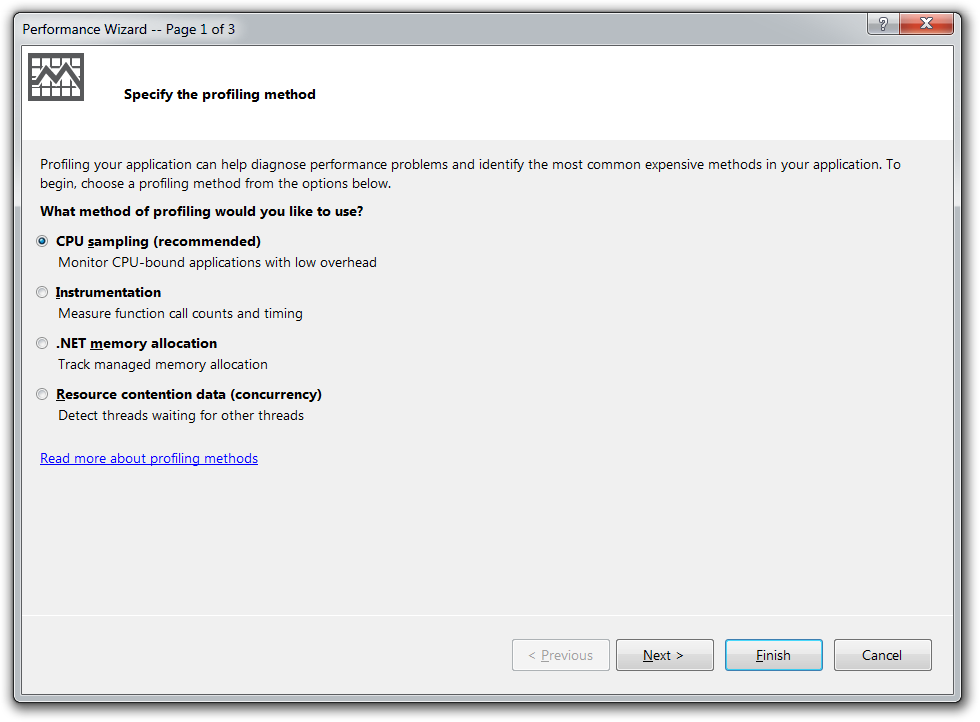
\includegraphics[scale=0.50]{figures/profiler/performance-wizard}
	\caption{De Performance Wizard}
	\label{performance-wizard}
\end{figure}

Wanner het programma klaar is met uitvoeren worden de resultaten geanalyseerd.
Als dat klaar is krijg je een algemeen overzicht van de resultaten.
Eerst en vooral zie je een grafiek met het CPU-gebruik doorheen de uitvoeringstijd van de applicatie.
Daaronder zie je de \emph{Hot Paths}, dat zijn de functies die verantwoordelijk zijn voor het grootste deel van de uitvoeringstijd.
Waar wij in geïnteresseerd zijn is hieraan gerelateerd: de \emph{Call Tree View}.
Die geeft je een boomstructuur van functies die elkaar oproepen en enkele belangrijke statistieken:
hoeveel keer een functie werd opgeroepen en hoeveel tijd de functie gemiddeld nodig had om uit te voeren,
dit zowel procentueel (ten opzichte van de totale uitvoeringstijd) als in absolute tijd.

De call tree van de SNMP Data Retriever kun je zien in \cref{call-tree}.
Hierbij werd de \emph{Main} functie opengeklapt. %TODO: Koppelteken
Je kunt functies verder open klappen om te zien welke andere functies worden opgeroepen en hun aandeel in de uitvoeringstijd analyseren.
Dit kan verder gaan tot je atomaire functies krijgt die geen andere functies meer oproepen.

In de call tree zie je naast de functienaam een aantal verschillende kolommen. Hieronder volgt de lijst van de kolommen en hun betekenis.

\begin{itemize}
	\item \textbf{Number of calls:}
		dit spreekt vrij voor zichzelf. Dit is het aantal keren dat een functie opgeroepen werd.
	\item \textbf{Elapsed Inclusive Time \%:}
		dit is het percentage van de uitvoeringstijd dat werd gespendeerd in deze functie en zijn kinderen.
	\item \textbf{Elapsed Exclusive Time \%:}
		dit is het percentage van de uitvoeringstijd dat uitsluitend in deze functie werd gespendeerd, dus \emph{exclusief} zijn kinderen.
	\item \textbf{Avg Elapsed Inclusive Time:}
		dit is de gemiddelde uitvoeringstijd in milliseconden van deze functie en zijn kinderen.
	\item \textbf{Avg Elapsed Exclusive Time:}
		dit is de gemiddelde uitvoeringstijd in milliseconden van uitsluitend deze functie, dus weer \emph{exclusief} zijn kinderen.
		\todo{Check of er geen pagebreak is op de individuele items.}
\end{itemize}

\begin{figure}[h]
	\centering
	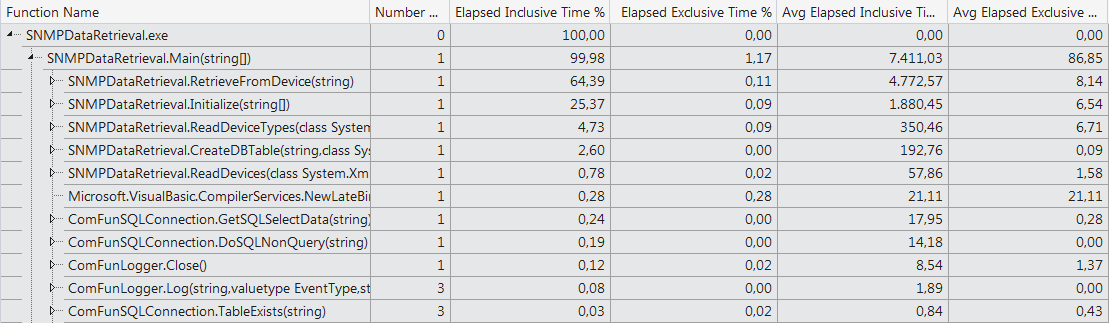
\includegraphics[scale=0.50]{figures/profiler/call-tree}
	\caption[De Call Tree]{De Call Tree. De kolommen van links naar rechts:
		\emph{Function Name},
		\emph{Elapsed Inclusive Time \%},
		\emph{Elapsed Exclusive Time \%},
		\emph{Avg Elapsed Inclusive Time},
		\emph{Avg Elapsed Exclusive Time}.}
	\label{call-tree}
\end{figure}

\subsubsection{De resultaten}

Voor het wegschrijven van de resultaten van de SNMP Data Retriever installeren we een lokale databank.
\todo{Vertellen we waarom?}
De retriever verwacht een MySQL databank, maar wij kiezen voor een MariaDB-installatie.
Omdat MariaDB een drop-in vervanging is voor MySQL is dat echter geen probleem.
Op het moment van installatie was de laatste stabiele versie 5.5.33a.

We doen een walk van 2 \glspl{oid} op een enkele productieswitch. Dit zal ons 443 objecten opleveren,
waarvan 441 die voor ons relevant zijn. Volgens de profiler doet de retriever daar ongeveer 7,4 seconden over.
De call tree van de retriever hebben we voor de leesbaarheid in een tabel gegoten (zie \cref{call-tree-main}).
De functies met een extreem kleine uitvoeringstijd (minder dan 0,01\%) hebben we achterwege gelaten.
De kolommen die je ziet zijn de functie, het aantal oproepen, de \emph{inclusieve} tijd als percentage van de totale uitvoeringstijd en
de gemiddelde \emph{inclusieve} tijd in milliseconden.

% Loglevel 2
\begin{table}[h]
	\centering
	\begin{tabular}{@{}lrrr@{}}
		\toprule
		Functie                                                  & Calls & Tijd (\%) & Tijd (ms) \\ \midrule
		SNMPDataRetrieval.RetrieveFromDevice                     & 1     & 64,39     & 4.772,57  \\
		SNMPDataRetrieval.Initialize                             & 1     & 25,37     & 1.880,45  \\
		SNMPDataRetrieval.ReadDeviceTypes                        & 1     & 4,73      & 350,46    \\
		SNMPDataRetrieval.CreateDBTable                          & 1     & 2,60      & 192,76    \\
		SNMPDataRetrieval.ReadDevices                            & 1     & 0,78      & 57,86     \\
		Microsoft.VisualBasic.CompilerServices.NewLateBinding.L… & 1     & 0,28      & 21,11     \\
		ComFunSQLConnection.GetSQLSelectData                     & 1     & 0,24      & 17,95     \\
		ComFunSQLConnection.DoSQLNonQuery                        & 1     & 0,19      & 14,18     \\
		ComFunLogger.Close                                       & 1     & 0,12      & 8,54      \\
		ComFunLogger.Log                                         & 3     & 0,08      & 1,89      \\
		ComFunSQLConnection.TableExists                          & 3     & 0,03      & 0,84      \\ \bottomrule
	\end{tabular}
	\caption{De call tree van de Main methode} %TODO: Koppelteken
	\label{call-tree-main}
\end{table}

\subsubsection{RetrieveFromDevice}

\todo[inline]{Titel: functienaam (RetrieveFromDevice) of oplossing/onderdeel/probleem (Bulk requests). \\
Hier maakt het weinig uit maar bij het volgende deel wel: Initialize of Logging (wat het probleem meteen weggeeft).}

We beginnen met de functie die het meeste tijd in beslag neemt: de \emph{RetrieveFromDevice} functie. %TODO: Koppelteken
Zoals de naam al verklapt gaat het hier om de methode die de requests stuurt om de gevraagde gegevens op te halen van de verschillende toestellen.

\todo[inline]{Hoort de uitleg over de werking van de SNMP Data Retriever hier?}
De manier waarop dit gebeurt is als volgt:
voor elk toestel dat ondervraagd moet worden wordt er een aparte thread gestart, met een maximum van 50 threads.
Elk van die threads zal alle gegevens opvragen die opgevraagd moeten worden voor dat toesteltype. \todo{Toesteltypes al vermeld?}
Wanneer een thread klaar is met gegevens opvragen wordt de thread verwijderd.
Indien er nog toestellen zijn die nog moeten ondervraagd worden, zal er dan een nieuwe thread opgestart worden voor het volgende toestel. \todo{Volledige uitleg over thread management geven of later uitleggen bij verbeteringen?}
Dit gaat zo door tot alle toestellen zijn ondervraagd.

In \cref{snmp-operaties} werden de verschillende SNMP operaties besproken waarmee men
gegevens kan opvragen. De originele versie van de SNMP Data Retriever die we eerst testen maakt gebruik van
GET-requests voor enkelvoudige gegevens en GETNEXT-requests om een SNMP walk te doen van 
een ganse deelboom.

De call tree van de RetrieveFromDevice functie zie je in \cref{call-tree-retrievefromdevice}. %TODO: Koppelteken
De twee belangrijkste methoden hier zijn de \emph{SyncRequest} en de \emph{InsertResultRow} methoden. %TODO: Koppelteken
SyncRequest maakt deel uit van de \emph{SnmpSource} bibliotheek. %TODO: Koppelteken
Dit is de third party bibliotheek waarvan gebruik gemaakt wordt om alle SNMP interacties af te handelen. %TODO: Koppelteken
De SyncRequest methode wordt gebruikt om synchroon een request te versturen.
Het feit dat de request synchroon gebeurt wil zeggen dat de code wacht op het antwoord alvorens verder te gaan.
We zien dat de methode 443 keer is opgeroepen dus dat wil zeggen dat er 443 requests verstuurd zijn geweest.
Gemiddeld deed een request er een kleine 10 milliseconden over, allen samen goed voor bijna 60\% (oftewel 4,28 seconden) van de totale uitvoeringstijd.

\begin{table}[h]
	\centering
	\begin{tabular}{@{}lrrr@{}}
		\toprule
		Functie                                                  & Calls & Tijd (\%) & Tijd (ms) \\ \midrule
		SnmpSource.SnmpSession.SyncRequest                       & 443   & 57,74     & 9,66      \\
		SNMPDataRetrieval.InsertResultRow                        & 441   & 3,75      & 0,63      \\
		SnmpSource.SnmpSession..ctor                             & 1     & 1,85      & 137,38    \\
		Microsoft.VisualBasic.CompilerServices.NewLateBinding.L… & 445   & 0,42      & 0,07      \\
		ComFunSQLConnection.TableContainsColumn                  & 2     & 0,12      & 4,43      \\
		ComFunLogger.Log                                         & 451   & 0,07      & 0,01      \\
		SnmpSource.SnmpPdu..ctor                                 & 1     & 0,05      & 3,84      \\
		Microsoft.VisualBasic.CompilerServices.Conversions.ToBo… & 2     & 0,04      & 1,59      \\
		Microsoft.VisualBasic.CompilerServices.NewLateBinding.L… & 6     & 0,04      & 0,52      \\
		SnmpSource.SnmpVariable.CreateSnmpVariable               & 443   & 0,02      & 0,00      \\ \bottomrule
	\end{tabular}
	\caption{De call tree van de RetrieveFromDevice methode} %TODO: Koppelteken
	\label{call-tree-retrievefromdevice}
\end{table}

\todo[inline]{Theoretische resultaten? (Adhv. testen met VirtualBox \& iMinds Switchen)}

\todo[inline]{Aanvullen. Implementeren van BULK requests.}

\subsubsection{Initialize}
\todo{Titel ok?}
\todo[inline]{Herschrijf begin van stuk over logging framework.}
Het eerste wat er ons opvalt als we de call tree bekijken is dat de \emph{Initialize} methode 25\% van de
uitvoeringstijd voor zijn rekening neemt.
Rijst de vraag wat deze functie juist doet dat ze zoveel tijd nodig heeft.

We klappen de Initialize methode open om de boosdoeners te zoeken.
De functies van de Initialize methode vind je terug in \cref{call-tree-initialize}.
We zien twee oproepen naar een \emph{Log} methode die er gemiddeld bijna een seconde over doet \emph{per oproep}! %TODO: Koppelteken

\begin{table}[h]
	\centering
	\begin{tabular}{@{}lrrr@{}}
		\toprule
		Functie                                                   & Calls & Tijd (\%) & Tijd (ms) \\ \midrule
		ComFunLogger.Log                                          & 2     & 20,97     & 777,30    \\
		ComFunSQLConnection..ctor                                 & 1     & 3,51      & 259,97    \\
		ComFunLogger.set\_LogFile                                 & 1     & 0,19      & 13,87     \\
		System.Configuration.ConfigurationManager.get\_AppSettin… & 12    & 0,16      & 0,99      \\
		Microsoft.VisualBasic.CompilerServices.Conversions.ToIn…  & 2     & 0,15      & 5,58      \\
		ComFunLogger.Log                                          & 4     & 0,13      & 2,41      \\
		ComFunLogger.Log                                          & 3     & 0,06      & 1,59      \\
		ComFunLogger.Log                                          & 2     & 0,05      & 1,87      \\
		ComFun.NetworkMiningCopyRightStatement                    & 1     & 0,03      & 2,03      \\
		ComFunLogger..ctor                                        & 1     & 0,01      & 1,10      \\ \bottomrule
	\end{tabular}
	\caption{De call tree van de Initialize methode} %TODO: Koppelteken
	\label{call-tree-initialize}
\end{table}

De \emph{ComFunLogger} is een stuk code die gebruikt wordt om te loggen naar een tekstbestand.
De naam komt van het feit dat ze een gemeenschappelijk stuk code is die over meerdere projecten kan
gebruikt worden: \emph{common functions}, of \emph{ComFun} voor kort.
Maar een functie die loggegevens wegschrijft naar een bestand hoort niet zo lang te duren.
I/O operaties zijn kostelijk, maar niet \emph{zo} kostelijk. %TODO: Koppelteken
Als we de functie helemaal openklappen in \cref{call-tree-performancecounter} vinden we de echte dader:
een constructor van \emph{System.Diagnostics.PerformanceCounter}.
Een performance counter wordt gebruikt voor het monitoren van systeemcomponenten zoals
processoren, geheugen en netwerk I/O. Als je ze gebruikt in je applicatie kunnen ze je %TODO: Koppelteken
informatie geven over de performantie van je programma.\cite{performance-counters-intro}
De ComFunLogger gebruikt ze om het geheugengebruik te meten en weg te schrijven in de logbestanden.

\begin{figure}[h]
	\centering
	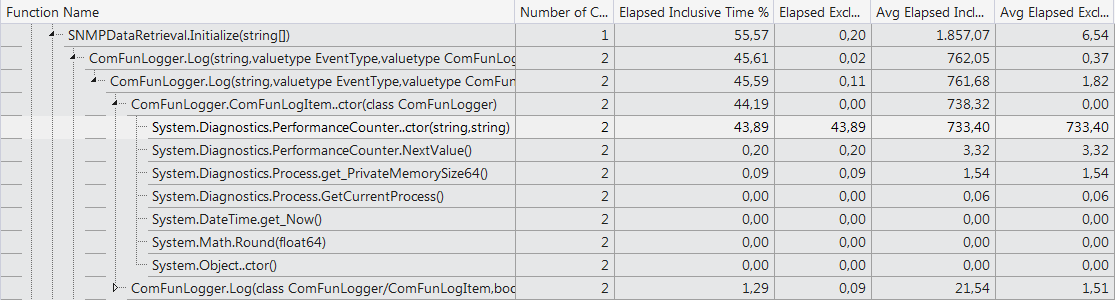
\includegraphics[scale=0.50]{figures/profiler/call-tree-performancecounter}
	\caption{De call tree van de Log methode}
	\label{call-tree-performancecounter}
\end{figure}

\todo[inline]{Herlees mij.}

Als oplossing werd ervoor gekozen om een alternatieve \emph{logging framework} te gebruiken.
Dit lijkt een drastische maatregel (en dat is het ook), maar daar zijn goede redenen voor.
Er zijn een heleboel gratis en open-source logging frameworks die reeds hun nut en kunnen bewezen hebben.
Zij zijn \emph{tried and true} oplossingen voor een algemeen probleem. \todo{Het zijn...}
Het is dus ook in de beste interesse voor een bedrijf om hiervoor te kiezen. \todo{Correcte zin?}
Financiëel is het een goede oplossing want de software is al ontwikkeld en is bewezen dat ze werkt.
Dit spaart tijd en geld uit voor de ontwikkeling van een eigen oplossing.
De software is gratis in gebruik dus er zijn geen licentiekosten aan verbonden.
Er zijn ook geen of lage onderhoudskosten. De software wordt al ingezet in zeer diverse omgevingen dus is al zeer uitgebreid.
De kans dat de software een bepaalde functionaliteit mist is dus klein.
En als er iets moet toegevoegd worden beschik je ook over de broncode.

Ook vanuit technisch opzicht is het een goede keuze.
Zoals gezegd heeft de software al zijn nut bewezen in diverse omgevingen.
In het specifieke geval van de ComFunLogger biedt een \emph{third party} oplossing ook een heleboel
extra flexibiliteit en features. Zo kan je loggen naar meerdere outputs en zijn er meerdere mogelijke outputs beschikbaar.
Je kunt bijvoorbeeld loggen naar tekstbestanden, consolevensters, databanken, enzovoort.

De twee belangrijkste redenen echter zijn het feit dat ze ontwikkeld zijn om een zo klein mogelijke performantieimpact te hebben en
dat de implementatie zeer simpel is.
Zo was het veel sneller om een ander logging framework te gebruiken dan om bekend te raken met de bestaande loggingcode en die te optimaliseren.

De keuze is uiteindelijk gevallen op Apache log4net en is gebaseerd op waarschijnlijk het bekendste logging framework voor java: Apache log4j.
Bij de keuze werd rekening gehouden met de performantieimpact en de features van de verschillende logging frameworks.\footnote{
	Een vergelijking tussen de bekendste logging frameworks voor .NET vind je 
	terug in de bronnenlijst bij bron \cite{logging-frameworks-and-performance} en \cite{logging-frameworks}.}



\todo[inline, caption={}]{

\begin{itemize}
	\item Waarom zijn er twee instanties nodig van de PerformanceCounter?
	\item Onderzoek op het internet leert ons dat PerformanceCounters hele kostelijke objecten zijn om aan te maken. Bron/citaat?
	\item x Oplossing: alternatieve loggingframework. Maar waarom heb je hiervoor gekozen ipv de huidige aan te passen?
	\item x Performantieredenen: ik heb een tried \& true logging framework opgezocht met nadruk op een minimale performantieimpact.
	\item x Plus de implementatie is ook sneller. Dan moet ik niet mijzelf bekend maken met de oude loggingcode en heb ik maar het 
		nieuwe loggingframework te includeren en alle logcalls te vervangen, wat vrij snel gebeurd is.
	\item x Lagere onderhoudskosten
	\item x Geen licentiekosten
	\item x Als leuke bonus krijg je er ook een heleboel extra features bij zoals logging naar meerdere outputs en meer outputformaten. (extra flexibiliteit)
	\item x Denk aan textfile, XML file, DB file, consoleuitvoer, etc.
	\item Nadeel: hoe groot is de extra code/binary van dit loggingframework? Andere nadelen?
\end{itemize}

}

\subsection{Tabellen rij per rij opvragen i.p.v. kolom per kolom}

\todo[inline]{Betere/kortere titel?}

\todo[inline, caption={}]{Vraag: waarom zou dit sneller zijn??? \\
Als je graag rij per rij LEEST zou kan je gebruik maken van het \textbf{smptable commando}.
Deze zorgt voor de correcte alignering en houdt rekening met indexen en gaten in de tabel.
Zie ook \textbf{http://www.net-snmp.org/wiki/index.php/TUT:snmptable}. \\
Zowel op VBox als iMinds Switchen \\

Caveats:

\begin{itemize}
	\item Goede integratie van MIB's vereist, want je moet weten welke kolommen er zijn en wat de indexering is
	\item Rekening houden met lege cellen/gaten in de tabel
	\item Als je de indexen op voorhand niet kent kun je maar een rij tegelijkertijd opvragen m.b.v. getnexts,
		Je kunt dus niet meer gegevens opvragen als er kolommen zijn in een request. Bulkrequests hebben daarentegen
		geen limiet op het aantal objecten (afgezien van de pakketgrootte natuurlijk).
\end{itemize}

}

\subsection{Impact van de fragmentatie van pakketten}

\todo{Titel: Snelheidsimpact?}


\section{Grootschalige benchmarks en experimenten}

\subsection{Testopstelling}

\todo[inline]{Testopstelling op de Virtual Wall.}

\subsection{Impact databankinteracties}

\subsection{Impact fragmentatie}

\subsection{Benchmarks uitvoeringstijd}

\todo[inline]{Oude versie vs. nieuwe versie}

\subsection{Benchmarks bandbreedte}

\subsubsection{SNMP Walk versus SNMP Bulk Requests}

\subsubsection{Invloed aantal ondervraagde nodes}

\todo[inline]{Verwijs voor dip in bandbreedte bij groot aantal nodes (>50) naar sectie CPU gebruik.}

\subsection{Benchmarks CPU-gebruik}

\todo[inline]{Onderzoek waarom verkeer \& CPU-verbruik dippen voor het einde (aantal threads daalt).}

\subsection{Benchmarks geheugenverbruik}